% Packages and Modules
\documentclass{report}
\usepackage{array}
\usepackage{amsmath}
\usepackage{hyperref}
\usepackage{graphicx}
\usepackage{circuitikz}
\usepackage[english]{babel}
\usepackage[utf8]{inputenc}
\usepackage[a4paper, margin=1in]{geometry}
\usepackage{tikz}

% Tikz config
\usetikzlibrary{calc}
\usetikzlibrary{positioning}

% Graphic config
\graphicspath{{./images/}}
\usetikzlibrary{shapes,arrows}
\numberwithin{equation}{section}

% Equation conditions
\newenvironment{conditions}
{\par\vspace{\abovedisplayskip}
\noindent\begin{tabular}{>{$}l<{$} @{${}={}$} l}}
        {\end{tabular}\par\vspace{\belowdisplayskip}}

% Title
\title{Synthesis of a Asynchronous Multilayer Perceptron on an FPGA}
\author{Fabian Franz}
\date{October 2020}

% Start of the document
\begin{document}
\maketitle

% Abstract
\begin{abstract}
\end{abstract}

% Introduction
\chapter{Introduction}
This project has the claim to design a low-power neural network on an FPGA.
To do so, the next sections give a brief introduction to the basic
principles of how such a neural network can be modeled.

\section{Perceptron}
A perceptron describes an analog model of a biological human cell in the
computer domain. This perceptron can be described with the following graphical
and mathematical expressions:

\begin{figure}[htbp]
    \begin{center}
        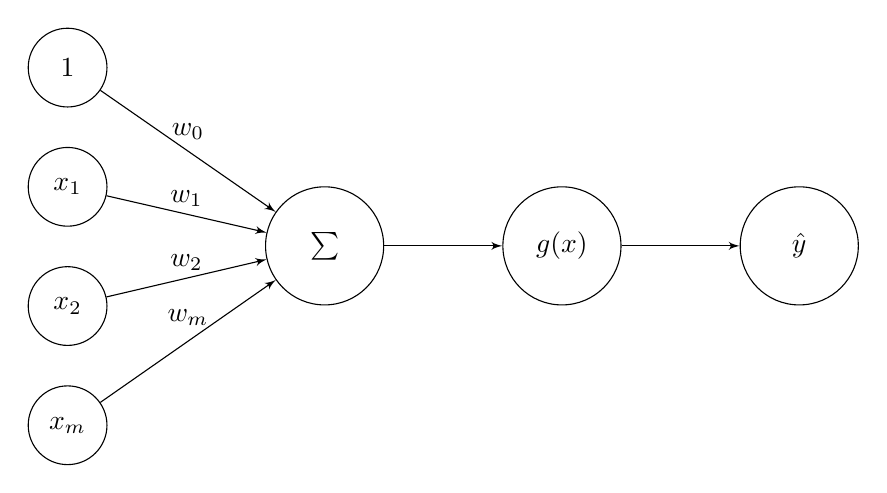
\begin{tikzpicture} [>=latex', node distance = 2cm]
            % Set primary nodes
            \tikzset{
                entity/.style={
                        rectangle,
                        draw
                    }
            }
            \tikzset{
                inputNode/.style={
                        draw,
                        circle,
                        minimum height=1cm
                    }
            }
            \tikzset{
                sumNode/.style={
                        draw,
                        circle,
                        minimum height=1.5cm
                    }
            }
            \tikzset{
                activationNode/.style={
                        draw,
                        circle,
                        minimum height=1.5cm
                    }
            }
            \tikzset{
                outNode/.style={
                        draw,
                        circle,
                        minimum height=1.5cm
                    }
            }
            % Placing nodes
            \node[inputNode](bias){$1$};
            \node[inputNode, below = 0.5cm of bias](x1){$x_1$};
            \node[inputNode, below = 0.5cm of x1](x2){$x_2$};
            \node[inputNode, below = 0.5cm of x2](xm){$x_m$};
            \node[sumNode, right = 2cm of x1, yshift = -0.75cm](sum){$\sum$};
            \node[activationNode, right = 1.5cm of sum](gx){$g(x)$};
            \node[outNode, right = 1.5cm of gx](out){$\hat y$};
            % Placing arrows
            \draw[->](bias) edge node[yshift = 0.25cm]{$w_0$} (sum);
            \draw[->](x1) edge node[yshift = 0.2cm]{$w_1$} (sum);
            \draw[->](x2) edge node[yshift = 0.2cm]{$w_2$} (sum);
            \draw[->](xm) edge node[yshift = 0.3cm]{$w_m$} (sum);
            \draw[->](sum) edge (gx);
            \draw[->](gx) edge (out);
        \end{tikzpicture}
    \end{center}
    \caption{Model of perceptron}
\end{figure}
\begin{equation}
    \hat y = g \Bigg( w_0 + \sum_{i=1}^{m}x_i w_i \Bigg)
\end{equation}
With:
\begin{conditions}
    g & Activation function \\
    w_o & Bias
\end{conditions}
In vector form:
\begin{equation}
    \hat y = g(W_0 + X^TW)
\end{equation}
With:
\begin{conditions}
    W & $\begin{pmatrix} w_1 \\ \vdots \\ w_m \end{pmatrix}$ , X = $\begin{pmatrix} x_1 \\ \vdots \\ x_m \end{pmatrix}$
\end{conditions}
As seen, in a conventional model of a perceptron every input of an
layer is multiplied by a weighting. It can be seen, that the implementation
of such a perceptron can be handled by given hardware architecture like GPU's
or matrix multiplier, because of the possibility to proceed every input matrix
and their associated weight matrix independently.

\section{Activation function}
The activation function of a perceptron has the purpose to determines the
behavior of the perceptron in response to external stimuli. There are different
kinds of activation functions which can be used for different purpuse. The most
common used one is the so called signoid function:

\section{Multilayer perceptron}

\section{Loss optimization}

% Method
\chapter{Method}

\section{Design}

\subsection{Hardware}

% Block diagram of board and wiring
\begin{figure}[htbp]
    \begin{center}
        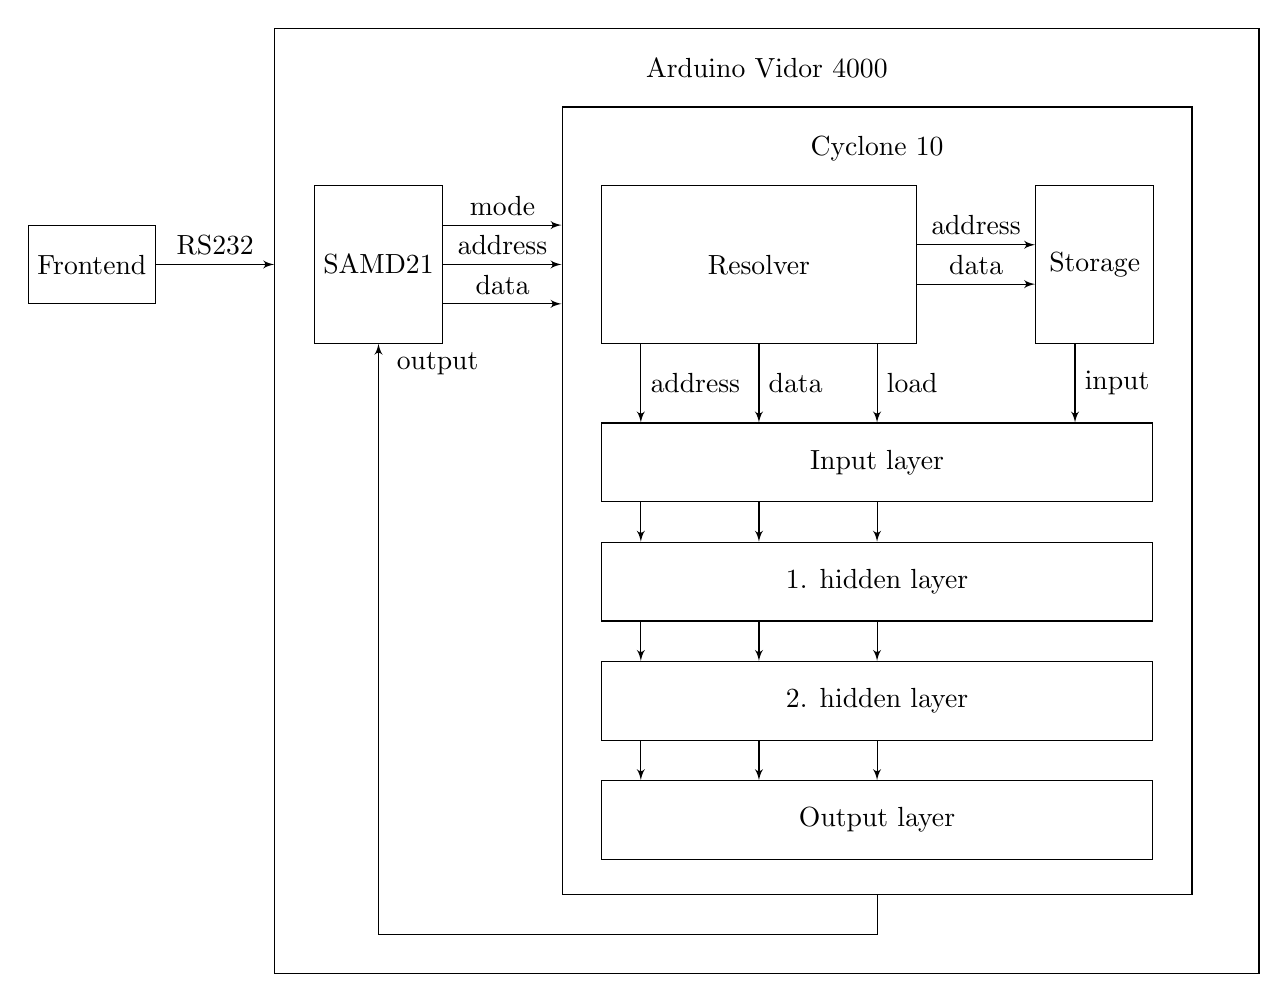
\begin{tikzpicture} [>=latex', node distance = 2cm]
            % Set primary nodes
            \tikzset{
                entity/.style={
                        rectangle,
                        draw
                    }
            }
            \tikzset{
                frontendNode/.style={
                        draw,
                        rectangle,
                        minimum height=1cm,
                        minimum width=1.5cm,
                    }
            }
            \tikzset{
                samd21Node/.style={
                        draw,
                        rectangle,
                        minimum height=2cm,
                        minimum width=1.5cm,
                    }
            }
            \tikzset{
                vidorNode/.style={
                        draw,
                        rectangle,
                        minimum height=12cm,
                        minimum width=12.5cm,
                        text depth = 11cm
                    }
            }
            \tikzset{
                fpgaNode/.style={
                        draw,
                        rectangle,
                        minimum height=10cm,
                        minimum width=8cm,
                        text depth = 9cm
                    }
            }
            \tikzset{
                resolverNode/.style={
                        draw,
                        rectangle,
                        minimum height=2cm,
                        minimum width=4cm
                    }
            }
            \tikzset{
                storageNode/.style={
                        draw,
                        rectangle,
                        minimum height=2cm,
                        minimum width=1.5cm
                    }
            }
            \tikzset{
                layerNode/.style={
                        draw,
                        rectangle,
                        minimum height=1cm,
                        minimum width=7cm
                    }
            }
            \tikzset{
                arrow/.style={
                        thick,
                        ->,
                        >=sealth
                    }
            }
            % Configure arrows
            \tikzstyle{arrow} = [thick, ->, >=stealth]
            % Placing nodes
            \node[frontendNode](frontend){Frontend};
            \node[vidorNode, right = 1.5cm of frontend, yshift = -3cm](vidor){Arduino Vidor 4000};
            \node[samd21Node, right = 2cm of frontend](samd21){SAMD21};
            \node[fpgaNode, right = 1.5cm of samd21, yshift = -3cm](fpga){Cyclone 10};
            \node[resolverNode, right = 2cm of samd21](resolver){Resolver};
            \node[storageNode, right = 1.5cm of resolver](storage){Storage};
            \node[layerNode, below = 1cm of resolver, xshift = 1.5cm](input){Input layer};
            \node[layerNode, below = 0.5cm of input](hidden1){1. hidden layer};
            \node[layerNode, below = 0.5cm of hidden1](hidden2){2. hidden layer};
            \node[layerNode, below = 0.5cm of hidden2](output){Output layer};
            % Draw arrows
            \draw[->](frontend.east) -- ++(1.5,0) node[midway,above]{RS232};
            \draw[->](samd21.east) ++(0,0.5) -- ++(1.5,0) node[midway,above]{mode};
            \draw[->](samd21.east) -- ++(1.5,0) node[midway,above]{address};
            \draw[->](samd21.east) ++(0,-0.5) -- ++(1.5,0) node[midway,above]{data};
            \draw[->](resolver.east) ++(0,0.25) -- ++(1.5,0) node[midway,above]{address};
            \draw[->](resolver.east) ++(0,-0.25) -- ++(1.5,0) node[midway,above]{data};
            \draw[->](resolver.south) ++(-1.5,0) -- ++(0,-1) node[midway,sloped,right, rotate=90]{address};
            \draw[->](resolver.south) ++(0,0) -- ++(0,-1) node[midway,sloped,right, rotate=90]{data};
            \draw[->](resolver.south) ++(1.5,0) -- ++(0,-1) node[midway,sloped,right, rotate=90]{load};
            \draw[->](storage.south) ++(-0.25,0) -- ++(0,-1) node[midway,sloped,right, rotate=90]{input};
            \draw[->](input.south) ++(-3,0) -- ++(0,-0.5) node[midway,sloped,right, rotate=90]{};
            \draw[->](input.south) ++(-1.5,0) -- ++(0,-0.5) node[midway,sloped,right, rotate=90]{};
            \draw[->](input.south) ++(0,0) -- ++(0,-0.5) node[midway,sloped,right, rotate=90]{};
            \draw[->](hidden1.south) ++(-3,0) -- ++(0,-0.5) node[midway,sloped,right, rotate=90]{};
            \draw[->](hidden1.south) ++(-1.5,0) -- ++(0,-0.5) node[midway,sloped,right, rotate=90]{};
            \draw[->](hidden1.south) ++(0,0) -- ++(0,-0.5) node[midway,sloped,right, rotate=90]{};
            \draw[->](hidden2.south) ++(-3,0) -- ++(0,-0.5) node[midway,sloped,right, rotate=90]{};
            \draw[->](hidden2.south) ++(-1.5,0) -- ++(0,-0.5) node[midway,sloped,right, rotate=90]{};
            \draw[->](hidden2.south) ++(0,0) -- ++(0,-0.5) node[midway,sloped,right, rotate=90]{};
            \draw[->](fpga.south) -- ++(0,-0.5) -| (samd21.south);
            \draw (samd21.south) ++(0.75,-0.25) node[]{output};
        \end{tikzpicture}
        \caption{Top level hardware model}
    \end{center}
\end{figure}
% Description of the Hardware


\subsection{Software}
% Block Diagram of Software Components
% Semi Code
% Structogram
\section{Procedure}

\subsection{Iplementation}
% Actual code fragments (Model)

\subsection{Validation}
% Actual code fragments (Testbench)
% Results

\chapter{Results}

\chapter{Discussion}

\bibliography{references}
\bibliographystyle{ieeetr}
\end{document}